\PassOptionsToPackage{svgnames}{xcolor}
\documentclass[12pt]{article}



\usepackage[margin=0.1in]{geometry}  
\usepackage{graphicx}             
\usepackage{amsmath}              
\usepackage{amsfonts}              
\usepackage{framed}               
\usepackage{amssymb} 
\usepackage{array}
\usepackage{amsthm}
\usepackage[nottoc]{tocbibind}
\usepackage{bm}
\usepackage{enumitem}


  \newcommand\norm[1]{\left\lVert#1\right\rVert}
\setlength{\parindent}{0cm}
\setlength{\parskip}{0em}
\newcommand{\Lim}[1]{\raisebox{0.5ex}{\scalebox{0.8}{$\displaystyle \lim_{#1}\;$}}}
\newtheorem{definition}{Definition}[section]
\newtheorem{theorem}{Theorem}[section]
\newtheorem{notation}{Notation}[section]
\theoremstyle{definition}
\DeclareMathOperator{\arcsec}{arcsec}
\DeclareMathOperator{\arccot}{arccot}
\DeclareMathOperator{\arccsc}{arccsc}
\DeclareMathOperator{\PV}{PV}
\DeclareMathOperator{\TV}{TV}
\DeclareMathOperator{\diff}{d}
\DeclareMathOperator{\expec}{E}
\DeclareMathOperator{\var}{Var}
\DeclareMathOperator{\cov}{Cov}
\DeclareMathOperator{\CE}{CE}
\DeclareMathOperator{\RP}{RP}
\newcommand\cf[1]{\mathbf{#1}}
\setcounter{tocdepth}{1}
\setcounter{section}{0}
\begin{document}

\title{Revision notes - MA4264}
\author{Ma Hongqiang}
\maketitle
\tableofcontents

\clearpage
\twocolumn
\section{Static Game of Complete Information}
\subsection{Pure Strategies}
\begin{definition}[Normal Form Representation]
\hfill\\\normalfont
The normal-form representation of an $n$-player game specifies the players'
\begin{itemize}
  \item \textbf{Strategy space} $S_1,\ldots, S_n$, and 
  \item their \textbf{payoff functions} $u_1, \ldots, u_n$, where $u_i: S_1\times \cdots\times S_n \to \mathbb{R}$.
\end{itemize}
We denote this game by $G=\{S_1,\ldots, S_n; u_1,\ldots, u_n\}$.\\
Let $(s_1,\ldots, s_n)$ be a combination of strategies, one for each player. Then $u_i(s_1,\ldots, s_n)$ is the payoff to player $i$ if for each $j=1,\ldots, n$, player $j$ chooses strategy $s_j$.
\end{definition}
\begin{definition}[Strictly Dominated]
\hfill\\\normalfont In a normal-form game $G=\{S_1,\ldots, S_n; u_1,\ldots, u_n\}$, let $s_i', s_i''\in S_i$. Strategy $s_i'$ is strictly dominated by strategy $s_i''$ if 
\[
u_i(s_i', s_{-i})<u_i(s_i'', s_{-i})\;\;\;\forall s_{-i}\in S_{-i}
\]
i.e., for each feasible combination of the other players' strategies, player $i$'s payoff from playing $s_i'$ is \textbf{strictly} less than the payoff from playing $s_i''$.
\end{definition}
Since rational players do not play strictly dominated strategies, we can eliminate these strictly dominated strategies iteratively, so as to reduce the dimension of $S_i, i=1,\ldots, n$, without removing the best response.
\begin{definition}[Best response]
\hfill\\\normalfont In the $n$-player normal-form game $G=\{S_1,\ldots, S_n; u_1,\ldots, u_n\}$, the \textbf{best response} for player $i$ to a combination of other player's strategies $s_{-i}\in S_{-i}$ is
\[
R_i(s_{-i})L=\arg\max_{s_i\in S_i}u_i(s_i, s_{-i})
\]
i.e., $R_i(s_{-i})$ is the \textit{set of best responses} by player $i$ to the other player's strategies $s_{-i}$.
\end{definition}
\textbf{Remark}: $R_i(s_{-i})\subset S_i$ can be an empty set, a singleton, or a finite or infinite set.
\begin{definition}[Nash Equilibrium]
\hfill\\\normalfont In the $n$-player normal-form game $G=\{S_1,\ldots, S_n; u_1,\ldots, u_n\}$, the strategies $(s_i^\ast, \ldots, s_n^\ast)$ is called a \textbf{Nash Equilibrium} if
\[
s_i^\ast \in R_i(s_{-i}^\ast) \;\;\;\forall i=1,\ldots, n
\]
equivalently, 
\[
u_i(s_i^\ast, s_{-i}^\ast) = \max_{s_i\in S_i} u_i(s_i, s_{-i}^\ast)\;\;\;\forall i=1,\ldots, n
\]
In other words, no player has incentive to deviate from Nash Equilibrium.
\end{definition}
To find a Nash Equilibrium in 2 player game, we can use graph. Let $G(R_i)$ denote the graph of $R_i$ defined by
\[
G(R_i)=\{(s_i, s_{-i})\mid s_i\in R_i(s_{-i}), s_{-i}\in S_{-i}\}
\]
Then $(s_i^\ast, \ldots, s_n^\ast)\in \cap_{i=1}^n G(R_i)$ if and only if it is in a Nash Equilibrium.\\
Specifically, in a 2-person game, we can compute the graph $R_1(s_2)$ and $R_2(s_1)$ and find the intersection.\\
If the game can be represented via a bimatrix, we can use the underline to denote the other player's best payoff to current player's strategy; do this for the 2 players and the cell with both underlined will be the best strategy.
\begin{theorem}[Relation between Nash Equilibrium and IESDS]
\hfill\\\normalfont If the strategies $(s_1^\ast, \ldots, s_n^\ast)$ are a Nash equilibrium in an $n$-player normal-form game $G=\{S_1,\ldots, S_n; u_1,\ldots, u_n\}$, then each $s_i^\ast$ cannot be eliminated in iterated elimination of strictly dominated strategies.
\end{theorem}
This implies: $\{\text{Nash Equilibria}\}\subseteq \{\text{Outcomes of IESDS}\}$.
\begin{theorem}
\hfill\\\normalfont In the $n$-player normal-form game $G=\{S_1,\ldots, S_n; u_1,\ldots, u_n\}$ where $S_1,\ldots, S_n$ are \textit{finite} sets, if IESDS eliminates all but the strategy $(s_1^\ast, \ldots, s_n^\ast)$, then these strategies are unique Nash equilibrium of the game.
\end{theorem}
In general, to compute Nash Equilibrium, find out expression $\pi_i(s_i, s_j)$ (usually in the form of piecewise functions), and take maximum to get a equation $s_i(s_j)$. Similarly, compute $\pi_j$ and get a equation $s_j(s_i)$. Find all intersections.
\subsection{Mixed Strategies}
\begin{definition}[Mixed Strategy]
\hfill\\\normalfont In the normal-form game $G=\{S_1,\ldots, S_n; u_1,\ldots, u_n\}$. Suppose $S_i=\{s_{i1}, \ldots, s_{iK}\}$. Then
\begin{itemize}
  \item Each strategy $s_{ik}$ in $S_i$is called a pure strategy for player $i$.
  \item A mixed strategy for player $i$ is a probability distribution $p_i(p_{i1}, \ldots, p_{iK})$, where $\sum_{k=1}^K p_{ik}=1$ and $p_{ik}\geq 0$.
\end{itemize}
We define the expected payoff for player $1$ to play mixed strategy $p_1:=(p_{11}, \ldots, p_{1J}$ is
\[
v_1(p_1,p_2)=\sum_{j=1}^J \sum_{k=1}^K p_{1j}p_{2k}u_1(s_{1j}, s_{2k})
\]
\end{definition}
\begin{definition}[Nash Equilibrium]
\hfill\\\normalfont In the two-player normal-form game $G=\{S_1,S_2; u_1,u_2\}$, the mixed strategies $(p_1^\ast, p_2^\ast)$ are a \textbf{Nash equilibrium} if each player's mixed strategy is a best response to the other player's mixed strategy, i.e.,
\[
v_1(p_1^\ast, p_2^\ast)\geq v_1(p_1, p_2^\ast)
\]
and 
\[
v_2(p_1^\ast, p_2^\ast)\geq v_2(p_1^\ast, p_2)
\]
for all probability distribution $p_1, p_2$ on $S_1, S_2$.
\end{definition}
Since it is completely known to us the value of $u_{1,2}(s_{1j}, s_{2k})$, the mixed strategy Nash Equilibrium only concerns solving the probability distribution. In a simplified setting where each player has only 2 strategies, let $p_1:=(r, 1-r)$ and $p_2=(q, 1-q)$, then 
\[
v_1(p_1, p_2)=rv_1(s_{11}, p_2)+(1-r)v_1(s_{12}, p_2)
\]
As you can see, $r$ here is dependent on $q$. So we can solve $r^\ast(q)$ by maximising the above equation. Specifically, we can have
\[
r^\ast(q)=\begin{cases}
1, &\text{ if }v_1(s_{11}, p_2)>v_1(s_{12}, p_2)\\
0, &\text{ if }v_1(s_{11}, p_2)<v_1(s_{12}, p_2)\\
[0,1], &\text{ if }v_1(s_{11}, p_2)=v_1(s_{12}, p_2)
\end{cases}
\]
And this is also true for $q^\ast(r)$. Then find intersections.
\begin{theorem}[Strategies eliminated by IESDS]
\hfill\\\normalfont If a pure strategy $s_{kj}\in S_{kj}$ is eliminated by IESDS, then this strategy will be played with zero probability $p_{kj}=0$, in any mixed strategy Nash Equilibrium. If there are only 2 strategies left for each player, then we can use the approach discussed before.
\end{theorem}
\begin{theorem}[Existence Theorem on Nash Equilibrium]
\hfill\\\normalfont In the $n$-player normal-form game $G=\{S_1,\ldots, S_n; u_1,\ldots, u_n\}$, if $n$ is \textit{finite} and $S_i$ is \textit{finite} for every $i$, then there eixsts at least one Nash equilibrium, possibly involving mixed strategies.
\end{theorem}
\section{Dynamic Games on Complete Information}
\begin{definition}[Dynamic Game of Complete and Perfect Information]
\hfill\\\normalfont A dynamic game of complete and perfect information is a game where
\begin{itemize}
  \item Players move in sequence, 
  \item (Perfect Information) All previous moves are observed before next move is chosen,
  \item (Complete Information): Payoffs are common knowledge
\end{itemize}
\end{definition}
Such games can be represented by a game tree.\\
\begin{figure}[h]
\centering
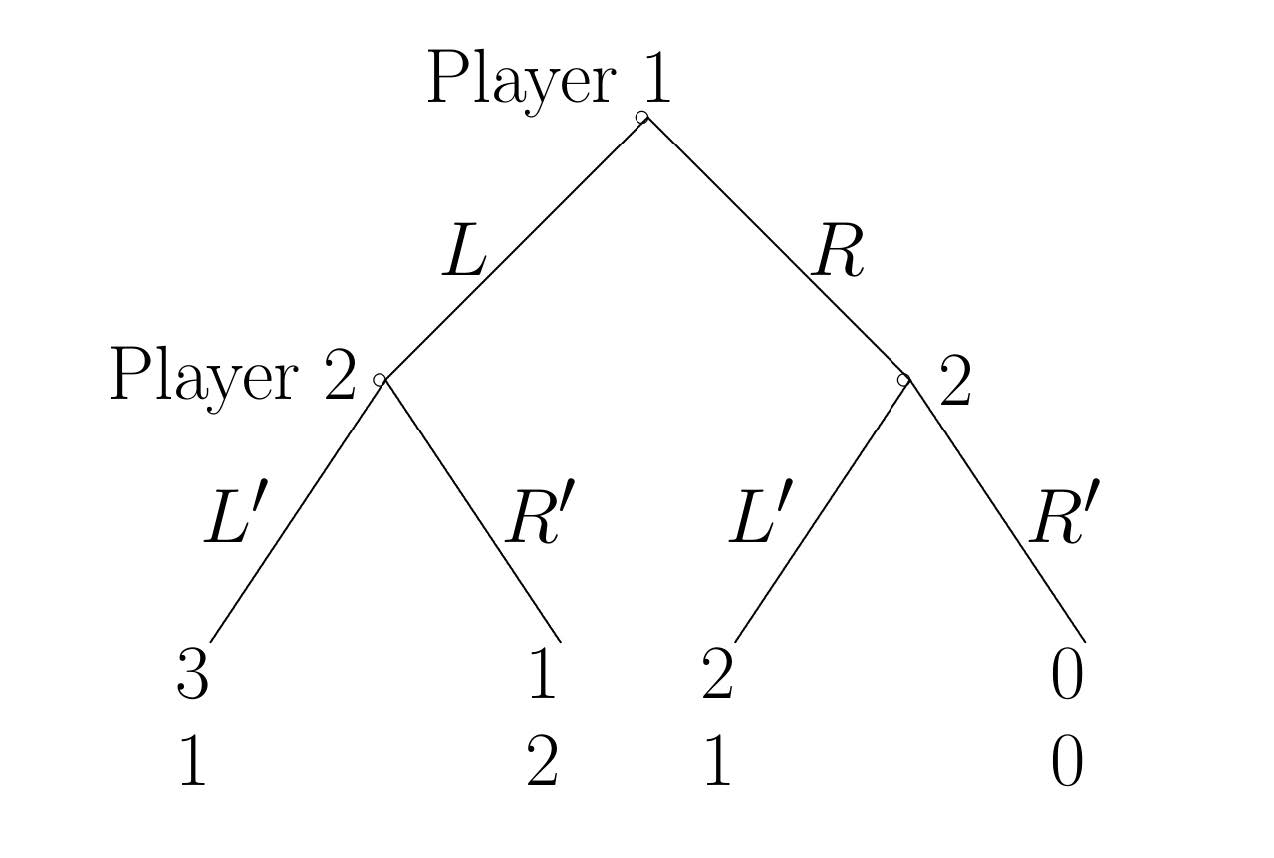
\includegraphics[width=0.4\textwidth]{2-1.jpg}
\end{figure}
In this chapter, we will see games with perfect, and imperfect information in sequence.
\begin{definition}[Backward Induction]
\hfill\\\normalfont The steps are as follow:
\begin{enumerate}
  \item At the second stage, player 2 observes the action chosen by player 1 at the first stage, say $a_1$, and then chooses an action by solving 
  \[
\arg \max_{a_2\in A_2} u_2(a_1, a_2)
  \]
  Assume this optimization problem has a unique solution, denoted by $R_2(a_1)$. This will be the best response.
  \item Player 1 will then solve $\max_{a_1\in A_1}u_1(a_1, R_2(a_1))$.\\
  Assume it has a unique solution $a_1^\ast$, we call $(a_1^\ast, R_2(a_1^\ast))$ the backwards-induction outcome of the game.
\end{enumerate}
\end{definition}
\subsection{Two Stage Games of Complete, Imperfect Information}
\begin{definition}[Subgame Perfect Outcome]
\hfill\\\normalfont 
Let players 1 and 2 simultaneously choose actions $a_1$ and $a_2$ from the feasible set $A_1, A_2$.\\
Let players 3 and 4 observe the outcome of the first stage $(a_1,a_2)$ and then simultaneously choose action $a_3, a_4$ from the feasible sets $A_3, A_4$ respectively.\\
Payoffs are $u_i(a_1,a_2,a_3,a_4)$ for $i=1,2,3,4$.\\
For each given $(a_1, a_2)$, player 3 and 4 try to find Nash equilibrium in stage 2. Assume the second-stage game has a unique Nash Equilibrium $(a_3(a_1, a_2), a_4(a_1,a_2))$, then player 1 and player 2 play a simultaneous-move game with payoffs $u_i(a_1,a_2,a_3(a_1,a_2), a_4(a_1,a_2))$. Suppose $(a_1^\ast, a_2^\ast)$ is the Nash equilibrium of the simultaneous-move game, then
\[
(a_1^\ast, a_2^\ast, a_3(a_1^\ast, a_2^\ast), a_4(a_1^\ast, a_2^\ast))
\]
is the \textbf{subgame-perfect} outcome of the 2-stage game.
\end{definition}
\begin{definition}[Extensive Form Representation]
\hfill\\\normalfont The \textbf{extensive form} representation of a game specifies
\begin{itemize}
  \item The players in teh game
  \item \begin{itemize}
  \item When each player has the move
  \item What each player can do at each move
  \item What each player knows at each of his or her move
  \item The payoff received by each player for each combinations of moves that could be chosen by the players
  \end{itemize}
\end{itemize}
\end{definition}
\begin{definition}[Information Set]
\hfill\\\normalfont An \textbf{information set} for a player is a collection of decision nodes satisfying:
\begin{itemize}
  \item The player needs to move at every node in the information set
  \item When the play of the game reached a node in the information set, the player with the move does not know which node in the set has been reached.
\end{itemize}
The second point impliees the player must have the \textbf{same set} of feasible actions at each decision node in an information set.
\end{definition}
A game is said to have \textbf{imperfect information} if some of its information sets are \textit{non-singletons}.\\
In an extensive-form game, a collection of decision nodes, which constitutes an information set, is connected by a dotted line.
\begin{definition}[Strategy]
\hfill\\\normalfont A \textbf{strategy} for a player is a \textbf{complete plan of actions}.\\
It specifies a feasible action for the player in every contingency in which the player might be called on to act. 
\end{definition}
\begin{definition}[Payoffs]
\hfill\\\normalfont In the extensive-form representation, payoffs are given for \textbf{each sequence of actions}, namely
\[
u_i(a_1,\ldots, a_m), \;\;\;i=1,\ldots, n
\]
where $a_1,\ldots, a_m$ are a sequence of actions.\\
Let $s=(s_1,\ldots, s_n)$ be a combination of strategies of $n$ players and $(a_1(s), \ldots, a_m(s))$ be the sequence of actions specified by $s(s_1,\ldots, s_n)$. Then the payoff received by playing $s=(s_1,\ldots, s_n)$ is
\[
\tilde{u}(s)=u(a_1(s), \ldots, a_m(s))
\]
where $s$ on LHS is strategy while the parameters in the RHS are actions taken.
\end{definition}
\begin{definition}[Normal Form and Nash Equilibrium]
The normal form of dynamic game specifies payoffs for each combination of \textbf{strategies}. Nash Equilibrium is obtained from teh normal-form representation.
\end{definition}
Remark: The Nash Equilibrium for dynamic games concerns about players' respective best \textbf{strategies}.\\
In general, we are interested in finding the Nash Equilibrium $(s_1, s_2)$ where $s_1\in A_1$ and $s_2=f:A_1\to A_2$. This means
\begin{itemize}
  \item Player 1 is interested in finding $\arg\max_{s_1}\tilde{u}_1(a_1=s_1, s_2^\ast)$
  \item Player 2 is interested in finding $\arg\max_{s_2}\tilde{u}_2(a_1, s_2)$ for each $a_1 \in A_1$
\end{itemize}
Here, although $R_2$ gives an $\arg\max$ of whatever player 1 plays, player 2 may \textit{not} follow this strategy.
\begin{theorem}\normalfont $(a_1^\ast, R_2)$ is a Nash equilibrium.
\end{theorem}
However, apart from $a_1^\ast$, there exists other Nash Equilibriums where player 1 not necessarily playing $a_1^\ast$.
\begin{definition}[Subgame Perfect Nash Equilibrium]
\hfill\\\normalfont A \textbf{subgame} in an extensive-form game
\begin{itemize}
  \item begins at a decision node $n$ that is a singleton information set (but is not the game's first decision node)
  \item includes all the decision and terminal nodes following node $n$ in teh game tree (but no nodes that do not follow $n$)
  \item does not cut any information sets (i.e., if a decision node $n'$ follows $n$ in the game tree, then all other nodes in the information set containing $n'$ must also follow $n$, and so must be included in teh subgame)
\end{itemize}
A Nash Equilibrium is \textbf{subgame-perfect} if the players' strategies constitute a Nash Equilibrium in every subgame.
\end{definition}
It can be shown that any finite dynamic game of complete information has a subgame-perfect Nash Equilibrium (which can be in mixed strategies).
\subsection{Infinitely Repeated Games}
Let $\pi_t$ be the payoff in stage $t$. Given a discount factor $\delta\in (0,1)$, the \textbf{present value} of sequence of payoff $\{\pi_1,\pi_2,\ldots\}$ is
\[
\pi_1+\delta\pi_2+\cdots = \sum_{t=1}^\infty \delta^{t-1} \pi_t
\]
Here the period 1 is un-discounted.
\begin{definition}[Infinitely Repeated Games]
\hfill\\\normalfont In the first stage, the player play the stage game $G$, and receive payoff $\pi_{1,1} and \pi_{2,1}$.\\
The game is repeated infinitely. In the $t$th stage, the players observe the actions chosen in the preceding $(t-1)$ stages, and then play $G$ to receive $(\pi_{1,t}, \pi_{2,t})$\\
The payoff of infinitely repeated game is the \textbf{presetn value} of sequence of payoffs:
\[
(\sum_{t=1}^\infty \delta^{t-1}\pi_{1,t}, \sum_{t=1}^\infty \delta^{t-1}\pi_{2,t})
\]
Playing the stage game $G$ does not mean having to play an equilibrium of $G$.\\
Denote by $A_{it}$ the action space of player $i$ in stage $t$. We have $A_t:=A_{1t}\times A_{2t}$.\\
A strategy by player $i$ is of the form $\{a_{i1}, a_{i2},\ldots\}$ where $a_{it}:A_1\times\cdots\times A_{t-1}\to A_{it}$.\\
The payoff received at stage $t$ is $\pi_{it}=u_i(a_{it}, a_{jt})$.
\end{definition}
Here, the non-cooperative strategy in Infinite Prisoner Dilemma is a Nash Equilibrium, whereas \textit{trigger strategy} is a Nash Equilibrium if and only if $\delta\geq \frac{1}{4}$. A trigger strategy chooses cooperation until being betrayed.
\begin{theorem}\normalfont Trigger strategy Nash Equilibrium($\delta\geq 1/4$) is subgame perfect.\end{theorem}

\end{document}

